\chapter{Sturing van de celcyclus en geprogrammeerde celdood}\label{ch:b3:cell-cycle-apoptosis}

Ongeveer honderd miljard cellen van het lichaam zullen vandaag met opzet
sterven, en honderd miljard zullen worden geboren om ze te vervangen;
de bekleding van de darm wordt elke vijf dagen vernieuwd en de rode
bloedcellen elke vier maanden. Een kikkervisje verliest zijn staart
zonder te bloeden; het vlies tussen de vingers van een menselijk embryo
verdwijnt in de achtste week; de helft van alle neuronen die ooit in
een hersenen worden gemaakt wordt vóór de geboorte gedood. Elk van
deze sterfgevallen wordt door de cel zelf volgens een programma
uitgevoerd, en elke geboorte wordt vergund door een besturingssysteem
dat op twee of drie punten in de cyclus beslist of de cel verder mag.
De twee programma's --- deling en zelfdoding --- vormen het onderwerp
van dit hoofdstuk. Zij zijn uitgezocht in gist, kikkereieren,
zee-egels en een worm met precies $1090$ somatische cellen waarvan er
precies $131$ sterven, en zij bleken bij de mens dezelfde, waar hun
falen aan de ene kant kanker is en aan de andere kant degeneratie.

\section{De motor van de cyclus}

\begin{definition}[Cyclines en cycline-afhankelijke kinasen]\label{def:b3:cell-cycle-apoptosis:cdk}
\index{cycline}\index{cycline-afhankelijk kinase}\index{anafase-bevorderend complex}\index{celcyclus}
De celcyclus --- G1, S (replicatie), G2, M (mitose) --- wordt
aangedreven door een familie eiwitkinasen, de \emph{cycline-afhankelijke
kinasen} (CDK's), waarvan de katalytische subeenheden de hele cyclus
aanwezig zijn maar alleen werkzaam wanneer zij aan een \emph{cycline}
zijn gebonden, een regulerende subeenheid waarvan de concentratie in
een vaste volgorde stijgt en daalt: cycline D met Cdk4/6 in G1 als
antwoord op groeifactoren, cycline E met Cdk2 bij de overgang G1/S,
cycline A met Cdk2 door S heen, cycline B met Cdk1 bij de intrede in de
mitose. Elk cycline-CDK-paar fosforyleert de eiwitten van zijn fase ---
replicatie-oorsprongen, lamines, condensines, de enzymen die de
spoelfiguur bouwen --- en elk wordt uitgezet door de vernietiging van
zijn cycline: ubiquitineligasen (SCF in G1/S, het
\emph{anafase-bevorderende complex}, APC/C, in de mitose) merken de
cyclines voor het proteasoom. De werking van Cdk1 wordt verder geregeld
door een remmende fosforylering die het kinase Wee1 aanbrengt en het
fosfatase Cdc25 verwijdert, en door kleine remmereiwitten (p21, p27,
p16) die de complexen binden. De cyclus is zo een geordende reeks
kinasegolven, waarbij elke golf eindigt in de afbraak van wat haar
voortbracht.
\end{definition}

\begin{proof}[Bewijsmateriaal]
Drie lijnen kwamen samen. Hartwell isoleerde in de jaren zeventig
temperatuurgevoelige \emph{cdc}-mutanten van bakkersgist, elk
gearresteerd in één stadium met een kenmerkende knopgrootte, en
definieerde \emph{Start}, het punt in G1 waarna een cel aan een cyclus
is gebonden. Nurse (jaren tachtig) vond in splijtgist dat \emph{cdc2}
de timing van de mitose bestuurde en dat het menselijke gen, in de
gist gebracht, de mutant redde: het kinase was Cdk1, geconserveerd van
gist tot mens. Hunt (1983) vond in zee-egeleieren een eiwit dat zich
elke cyclus ophoopte en bij elke deling abrupt werd vernietigd, en
noemde het \omterm{def:b3:cell-cycle-apoptosis:cdk}{cycline}. Het kikkerei had intussen een
``rijpingsbevorderende factor'' opgeleverd die elke kern de mitose in
dreef; het was \omterm{def:b3:cell-cycle-apoptosis:cdk}{cycline} B gebonden aan Cdk1. Rao en Johnson (1970)
hadden door cellen te versmelten laten zien dat een cel in S-fase een
G1-kern de replicatie in drijft, terwijl een G2-kern wacht --- het
cytoplasma draagt het signaal, en een gerepliceerde kern is niet tot
opnieuw repliceren te brengen.
\end{proof}

\begin{omfigure}
\begin{tikzpicture}[every node/.style={font=\scriptsize}, >=stealth]
  % cycle circle with phases
  \draw[very thick, omDef!50] (0,0) circle (2.2);
  \foreach \a/\b/\col/\lab/\r in {90/200/omDef!25/G1/1.55, 200/270/omProp!30/S/1.55, 270/315/omMeth!30/G2/1.55, 315/450/omThm!30/M/1.55} {
    \fill[\col] (0,0) -- (\a:2.2) arc[start angle=\a, end angle=\b, radius=2.2] -- cycle;
    \node[font=\small\bfseries] at ({(\a+\b)/2}:\r) {\lab};
  }
  \fill[white] (0,0) circle (1.0);
  \draw[very thick, omDef!50] (0,0) circle (2.2);
  % cyclin-CDK labels around
  \node[left, align=right] at (-2.4,1.2) {cycline D--Cdk4/6\\groeifactoren, Rb uit};
  \node[left, align=right] at (-2.4,-1.0) {cycline E--Cdk2\\oorsprongen vuren};
  \node[anchor=north east, align=right] at (-1.3,-2.2) {cycline A--Cdk2\\replicatie};
  \node[right, align=left] at (2.4,-1.0) {cycline B--Cdk1\\intrede in de mitose};
  \node[right, align=left] at (2.4,1.3) {APC/C vernietigt cycline B\\en securine: anafase, uitgang};
  % checkpoints as bars
  \foreach \a in {160,270,20} \draw[very thick, omThm] (\a:1.95) -- (\a:2.45);
  \node[align=center, anchor=south east] at (-1.2,2.35) {restrictiepunt:\\groeifactoren?};
  \node[align=left, anchor=west] at (2.55,0.35) {controlepunt van de spoelfiguur:\\alle kinetochoren gehecht?};
  \node[align=center, anchor=north] at (1.5,-2.55) {controlepunt G2/M:\\DNA intact?};
  \draw[->, thick] (0,0) ++(60:1.25) arc[start angle=60, end angle=30, radius=1.25];
\end{tikzpicture}

{\small De cyclus als een reeks golven van \omterm{def:b3:cell-cycle-apoptosis:cdk}{cycline} en CDK, elk beëindigd
door de vernietiging van haar \omterm{def:b3:cell-cycle-apoptosis:cdk}{cycline}, met de drie \omterm{def:b3:cell-cycle-apoptosis:checkpoints}{controlepunten} (rode
balken) waarbij de cel zich afvraagt of zij verder gaat.}
\end{omfigure}

\begin{theorem}[Een schakelaar en een vertraagde rem maken een oscillator]\label{thm:b3:cell-cycle-apoptosis:oscillator}
\index{relaxatieoscillator}\index{bistabiliteit!celcyclus}\index{hysterese}
Zij $A$ de werkzaamheid van \omterm{def:b3:cell-cycle-apoptosis:cdk}{cycline} B--Cdk1 en $C$ de hoeveelheid
\omterm{def:b3:cell-cycle-apoptosis:cdk}{cycline} B. Stel (i) dat bij vaste $C$ de grootheid $A$ snel naar een
evenwichtstoestand gaat die van $C$ afhangt via een positieve
terugkoppeling (werkzaam Cdk1 activeert zijn activator Cdc25 en remt
zijn remmer Wee1), zodat de evenwichtscurve $A^{*}(C)$ S-vormig is:
voor $C$ tussen twee drempels $C_{1} < C_{2}$ bestaan er zowel een lage
als een hoge toestand, en het systeem blijft op de tak waarop het zit
(\emph{hysterese}); en (ii) dat $C$ traag verandert, met een constante
snelheid $k_{s}$ wordt gemaakt en met snelheid $k_{d}A\,C$ wordt
afgebroken via het APC/C, dat werkzaam Cdk1 na enige vertraging
aanzet. Dan heeft het systeem geen stabiele evenwichtstoestand en
voert het een \emph{relaxatieoscillatie} uit: $C$ hoopt zich op de lage
tak op tot het $C_{2}$ voorbijgaat, $A$ springt naar de hoge tak (de
intrede in de mitose), de afbraak wint het van de aanmaak en $C$ daalt
tot het $C_{1}$ voorbijgaat, $A$ stort in naar de lage tak (de uitgang
uit de mitose), en de cyclus herhaalt zich. De periode wordt vooral
bepaald door de trage variabele: ongeveer $C_{2}/k_{s}$ voor de
stijging, plus de tijd om van $C_{2}$ tot $C_{1}$ af te breken.
\end{theorem}
\begin{proof}[Gedeeltelijk bewijs]
Een evenwichtstoestand van het paar zou $\mathrm{d}C/\mathrm{d}t = 0$
vergen, dat wil zeggen $k_{s} = k_{d}A^{*}(C)\,C$, in een punt op de
S-vormige curve. Op de lage tak is $A^{*}$ klein, dus geldt
$k_{d}A^{*}C < k_{s}$ voor $C$ tot aan $C_{2}$: het \omterm{def:b3:cell-cycle-apoptosis:cdk}{cycline} stijgt en
het systeem wordt van het einde van de tak gevoerd. Op de hoge tak is
$A^{*}$ groot, dus geldt $k_{d}A^{*}C > k_{s}$ voor $C$ tot aan
$C_{1}$: het \omterm{def:b3:cell-cycle-apoptosis:cdk}{cycline} daalt en het systeem wordt van dat einde gevoerd.
De enige kandidaat-evenwichtstoestand zou op de middelste, instabiele
tak liggen, en een punt daar stoot af; er is dus geen stabiele
evenwichtstoestand, en de baan, beperkt tot de twee stabiele takken en
de sprongen ertussen, doorloopt een cyclus. De tijd op de lage tak is
$\int \mathrm{d}C/(k_{s} - k_{d}A^{*}C) \approx C_{2}/k_{s}$ wanneer
$A^{*}$ klein is, en de tijd op de hoge tak is de kortere tijd om
$C_{2} - C_{1}$ met snelheid $k_{d}A^{*}_{\text{high}}C$ af te breken.
Het bestaan van de S-vormige curve uit de terugkoppeling van Cdc25 en
Wee1 wordt hier aangenomen; het is dezelfde bistabiliteit als bij het
zelfactiverende gen uit het boek van jaar~2, met nu een kinase als
snelle variabele en zijn \omterm{def:b3:cell-cycle-apoptosis:cdk}{cycline} als trage.
\end{proof}

\begin{omfigure}
\begin{tikzpicture}
\begin{axis}[
  width=6.6cm, height=5.6cm,
  axis lines=left,
  xmin=0, xmax=1.4, ymin=0, ymax=1.1,
  xlabel={cycline B, $C$}, ylabel={werkzaamheid van Cdk1, $A$},
  xlabel style={font=\small, at={(axis description cs:0.5,-0.12)}, anchor=north}, ylabel style={font=\small},
  tick label style={font=\scriptsize}, xtick={0.4,1.0}, xticklabels={$C_{1}$,$C_{2}$}, ytick=\empty,
  clip=false,
]
% S-shaped nullcline: two stable branches and a dashed unstable one
\addplot[very thick, omDef, smooth] coordinates {(0,0.02) (0.5,0.04) (0.9,0.07) (1.0,0.1)};
\addplot[very thick, omDef, dashed, smooth] coordinates {(1.0,0.1) (0.85,0.3) (0.7,0.5) (0.55,0.7) (0.4,0.9)};
\addplot[very thick, omDef, smooth] coordinates {(0.4,0.9) (0.6,0.94) (1.0,0.97) (1.4,0.98)};
\draw[->, very thick, omThm] (axis cs:0.05,0.15) -- (axis cs:0.98,0.15);
\draw[->, very thick, omThm] (axis cs:1.04,0.18) -- (axis cs:1.04,0.82);
\draw[->, very thick, omThm] (axis cs:0.98,0.84) -- (axis cs:0.42,0.84);
\draw[->, very thick, omThm] (axis cs:0.36,0.82) -- (axis cs:0.36,0.18);
\node[font=\scriptsize, omThm, anchor=south west] at (axis cs:0.36,0.24) {cycline hoopt zich op};
\node[font=\scriptsize, omThm, anchor=west] at (axis cs:1.07,0.5) {intrede};
\node[font=\scriptsize, omThm, anchor=south] at (axis cs:0.7,1.0) {APC/C breekt cycline af (mitose)};
\node[font=\scriptsize, omThm, anchor=east] at (axis cs:0.33,0.5) {uitgang};
\node[font=\scriptsize, omDef, anchor=north east] at (axis cs:1.38,0.95) {$A^{*}(C)$};
\end{axis}
\begin{axis}[
  at={(7.6cm,0)}, anchor=south west,
  width=6.6cm, height=5.6cm,
  axis lines=left,
  xmin=0, xmax=3, ymin=0, ymax=1.2,
  xlabel={tijd (cycli)}, ylabel={},
  xlabel style={font=\small, at={(axis description cs:0.5,-0.12)}, anchor=north},
  tick label style={font=\scriptsize}, xtick={0,1,2,3}, ytick=\empty,
  clip=false,
]
\addplot[very thick, omDef] coordinates {(0,0.4) (0.8,1.0) (0.95,0.4) (1.75,1.0) (1.9,0.4) (2.7,1.0) (2.85,0.4) (3,0.5)};
\addplot[very thick, omThm] coordinates {(0,0.05) (0.8,0.05) (0.8,0.95) (0.95,0.95) (0.95,0.05) (1.75,0.05) (1.75,0.95) (1.9,0.95) (1.9,0.05) (2.7,0.05) (2.7,0.95) (2.85,0.95) (2.85,0.05) (3,0.05)};
\node[font=\scriptsize, omDef, anchor=south west] at (axis cs:1.0,0.1) {cycline B};
\node[font=\scriptsize, omThm, anchor=south west] at (axis cs:1.0,1.0) {werkzaamheid van Cdk1};
\end{axis}
\end{tikzpicture}

{\small Links: het faseplat van de oscillator. De S-vormige curve is de
snelle evenwichtstoestand van Cdk1 bij elk cyclineniveau; de rode lus
is de cyclus --- trage ophoping langs de lage tak, een sprong bij
$C_{2}$, snelle afbraak langs de hoge tak, een sprong terug bij
$C_{1}$. Rechts: het bijbehorende tijdsverloop, een zaagtand van
\omterm{def:b3:cell-cycle-apoptosis:cdk}{cycline} en een blokgolf van kinase.}
\end{omfigure}

\begin{example}[Waarom het kikkerei een klok is]\label{ex:b3:cell-cycle-apoptosis:frog}
Een bevrucht kikkerei deelt zich twaalf keer in zes uur zonder groei,
zonder transcriptie en zonder \omterm{def:b3:cell-cycle-apoptosis:checkpoints}{controlepunten}, met tussenpozen van
\qty{30}{min}: het is de oscillator van de stelling die kaal draait, en
een extract van zijn cytoplasma in een reageerbuis blijft doorlopen,
met stijgend en dalend \omterm{def:b3:cell-cycle-apoptosis:cdk}{cycline}, zonder dat er iets te delen valt. Een
niet-afbreekbaar \omterm{def:b3:cell-cycle-apoptosis:cdk}{cycline} B toevoegen zet het extract vast in de mitose,
omdat $C$ nooit onder $C_{1}$ kan zakken; de cyclinesynthese blokkeren
zet het vast in de interfase. In een somatische cel is dezelfde motor
verpakt in de besturing van de volgende paragraaf, die haar bij de
drempels tegenhoudt tot aan de voorwaarden is voldaan, zodat de periode
een dag wordt in plaats van een half uur en onbeperkt lang kan zijn.
\end{example}

\section{Controlepunten}

\begin{definition}[Controlepunten]\label{def:b3:cell-cycle-apoptosis:checkpoints}
\index{controlepunt}\index{restrictiepunt}\index{controlepunt van de spoelfiguur}\index{replicatievergunning}
Een \emph{controlepunt} is een besturing die de cyclus bij een overgang
stillegt tot aan een voorwaarde is voldaan, door op de motor in te
grijpen --- door een CDK of een ubiquitineligase te remmen. Drie doen
het meest ertoe. Het \emph{restrictiepunt} laat in G1 (Start bij gist):
de cel gaat alleen verder als groeifactoren, voedingsstoffen en grootte
het toelaten; voorbij dat punt voltooit de cyclus zich zonder hen. Het
\emph{controlepunt G2/M}: beschadigd of niet-gerepliceerd DNA,
gemeld door de kinasen \omterm{def:b3:dna-repair:ddr}{ATM} en ATR uit \cref{ch:b3:dna-repair}, houdt
Cdc25 geremd en daarmee Cdk1 gefosforyleerd en inactief. Het
\emph{controlepunt van de spoelfiguur}: één enkele kinetochoor die niet
aan \omterm{def:b3:cytoskeleton-motility:filaments}{microtubuli} is gehecht maakt een diffundeerbare remmer (Mad2
gebonden aan Cdc20) die het APC/C uit houdt, zodat de anafase op het
laatste chromosoom wacht. Een vierde besturing kent geen wachtstap maar
is even streng: de \emph{replicatievergunning}. Oorsprongen worden
alleen in G1 met het MCM-helicase geladen, wanneer de CDK-werkzaamheid
laag is, en de ladingsfactoren worden vernietigd of geremd zodra de
S-fase begint, zodat elke oorsprong precies eenmaal per cyclus vuurt
--- de reden dat een G2-kern in de fusies van Rao en Johnson niet tot
repliceren te brengen was.
\end{definition}

\begin{proposition}[Het restrictiepunt is een schakelaar]\label{prop:b3:cell-cycle-apoptosis:rb}
\index{retinoblastoma-eiwit}\index{E2F}
Vroeg in G1 wordt de transcriptiefactor \emph{E2F}, die de genen van de
S-fase aandrijft (\omterm{def:b3:cell-cycle-apoptosis:cdk}{cycline} E, \omterm{def:b3:cell-cycle-apoptosis:cdk}{cycline} A, de replicatie-enzymen),
inactief gehouden door het \emph{\omterm{prop:b3:cell-cycle-apoptosis:rb}{retinoblastoma-eiwit}} Rb.
Groeifactoren zetten \omterm{def:b3:cell-cycle-apoptosis:cdk}{cycline} D aan, en \omterm{def:b3:cell-cycle-apoptosis:cdk}{cycline} D--Cdk4/6 begint Rb te
fosforyleren, waardoor een beetje E2F vrijkomt; E2F zet daarop \omterm{def:b3:cell-cycle-apoptosis:cdk}{cycline}
E aan, en \omterm{def:b3:cell-cycle-apoptosis:cdk}{cycline} E--Cdk2 fosforyleert Rb veel sterker --- een positieve
terugkoppeling die zich, eenmaal over een drempel, zonder verdere
groeifactor voltooit. De cel is het \omterm{def:b3:cell-cycle-apoptosis:checkpoints}{restrictiepunt} gepasseerd; E2F zet
ook zijn eigen gen aan. Het verlies van Rb, of van de Cdk4/6-remmer
p16, of de vermenigvuldiging van \omterm{def:b3:cell-cycle-apoptosis:cdk}{cycline} D, haalt de behoefte aan
groeifactor geheel weg, en alle drie komen vaak voor bij kanker
(\cref{ch:b3:cancer-biology}); geneesmiddelen die Cdk4/6 remmen worden
nu gebruikt tegen borstkankers die van deze schakelaar afhangen.
\end{proposition}

\begin{omfigure}
\begin{tikzpicture}[every node/.style={font=\scriptsize}, >=stealth]
  \node[draw, thick, rounded corners, fill=omProp!25, minimum width=2.2cm] (gf) at (0,2.2) {groeifactoren};
  \node[draw, thick, rounded corners, fill=omDef!20, minimum width=2.4cm] (cd) at (0,1.0) {cycline D--Cdk4/6};
  \node[draw, thick, rounded corners, fill=omThm!20, minimum width=1.6cm] (rb) at (3.8,1.0) {Rb};
  \node[draw, thick, rounded corners, fill=omMeth!25, minimum width=1.6cm] (e2f) at (7.2,1.0) {E2F};
  \node[draw, thick, rounded corners, fill=omDef!20, minimum width=2.4cm] (ce) at (7.2,-0.6) {cycline E--Cdk2};
  \node[draw, thick, rounded corners, fill=gray!15, align=center, minimum width=2.6cm] (s) at (10.8,1.0) {genen van de S-fase:\\cycline A, MCM, \dots};
  \draw[->, thick] (gf) -- (cd);
  \draw[-|, thick, omThm] (cd) -- (rb) node[midway, above, font=\tiny] {fosforyleert};
  \draw[-|, thick, omThm] (rb) -- (e2f) node[midway, above, font=\tiny] {houdt inactief};
  \draw[->, thick] (e2f) -- (s);
  \draw[->, thick] (e2f) -- (ce) node[midway, right] {zet aan};
  \draw[-|, thick, omThm] (ce.west) -- ++(-2.2,0) |- (rb.south) node[pos=0.25, below] {fosforyleert Rb verder};
  \draw[->, thick, omMeth!70!black] (e2f.north) .. controls (6.0,2.2) and (6.8,2.2) .. (e2f.north east) node[pos=0.5, above] {zet zijn eigen gen aan};
  \node[draw, thick, rounded corners, fill=omThm!10] (p16) at (0,-0.6) {p16}; \draw[-|, thick, omThm] (p16) -- (cd);
\end{tikzpicture}

{\small Het \omterm{def:b3:cell-cycle-apoptosis:checkpoints}{restrictiepunt}. Groeifactoren beginnen de fosforylering van
Rb, die een beetje E2F vrijmaakt; E2F zet \omterm{def:b3:cell-cycle-apoptosis:cdk}{cycline} E aan, waarvan het
kinase Rb verder fosforyleert --- een positieve terugkoppeling die de
overgang voltooit en haar onafhankelijk maakt van het beginsignaal. De
balken duiden remming aan.}
\end{omfigure}

\begin{proposition}[De anafase is een beslissing door eiwitafbraak]\label{prop:b3:cell-cycle-apoptosis:anaphase}
\index{securine}\index{separase}\index{cohesine}
Zusterchromatiden worden vanaf de S-fase bijeengehouden door ringen van
\emph{cohesine}. In de metafase, wanneer elke kinetochoor is gehecht en
het \omterm{def:b3:cell-cycle-apoptosis:checkpoints}{controlepunt van de spoelfiguur} zwijgt, ubiquitineert het APC/C met
zijn activator Cdc20 twee eiwitten: \omterm{def:b3:cell-cycle-apoptosis:cdk}{cycline} B, waarvan het verlies Cdk1
uitschakelt en de cel de mitose laat verlaten, en \emph{securine},
waarvan het verlies het protease \emph{separase} vrijmaakt, dat
cohesine doorknipt. Alle zusterparen gaan binnen enkele seconden van
elkaar uiteen, door de spoelfiguur naar de polen getrokken, en de cel
deelt zich met een ring van actine en \omterm{def:b3:cytoskeleton-motility:motors}{myosine}~II die wordt gebouwd waar
de middenzone van de spoelfiguur het de cortex zegt (via RhoA). De
beslissing is onomkeerbaar omdat zij op eiwitafbraak berust: een
doorgeknipt cohesine kan niet opnieuw worden gebouwd, en het afgebroken
\omterm{def:b3:cell-cycle-apoptosis:cdk}{cycline} moet opnieuw worden gemaakt. Fouten hier --- een chromosoom
naar de verkeerde pool getrokken, een anafase die vóór de laatste
hechting begint --- leveren aneuploïde dochters op, de meest
voorkomende chromosoomafwijking van tumoren en van miskramen.
\end{proposition}

\begin{omfigure}
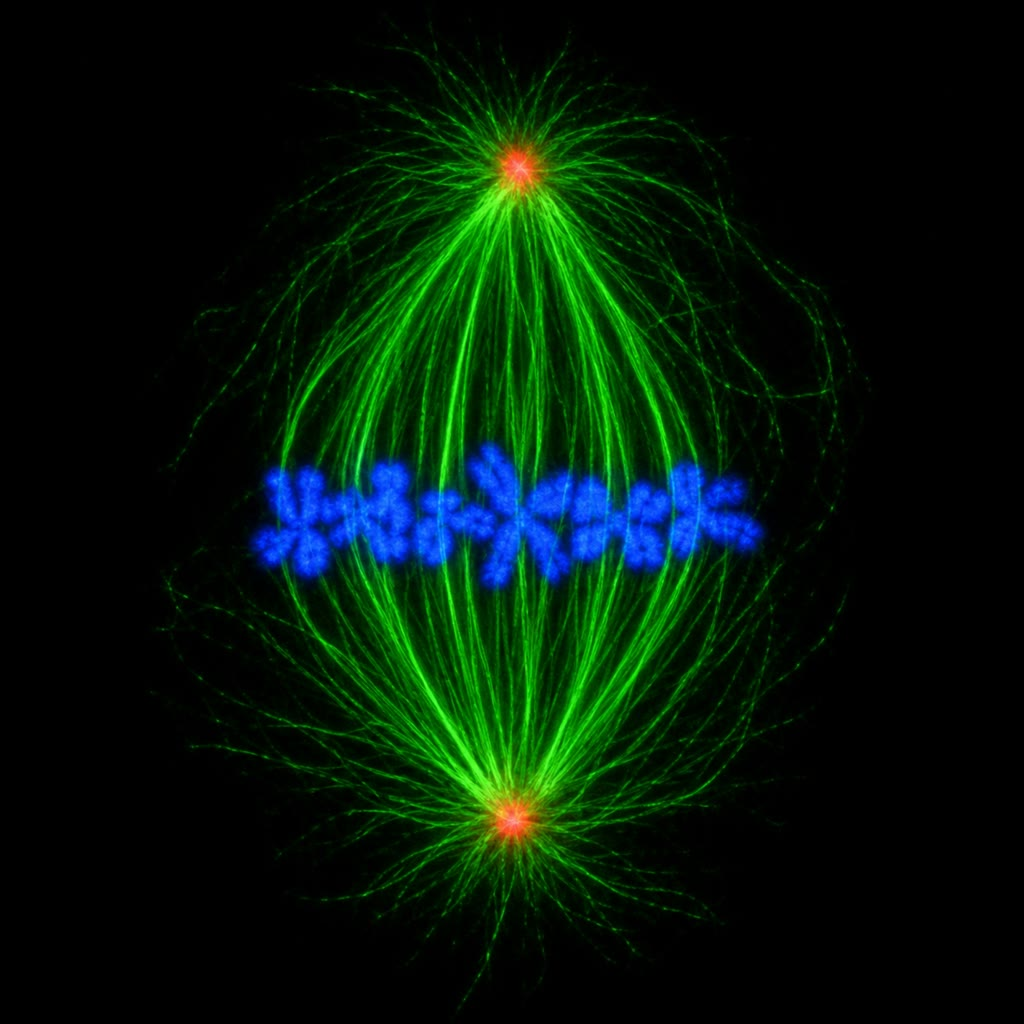
\includegraphics[width=0.36\linewidth]{images/book5/ai/b5-10-mitotic-spindle.jpg}\hspace{0.04\linewidth}
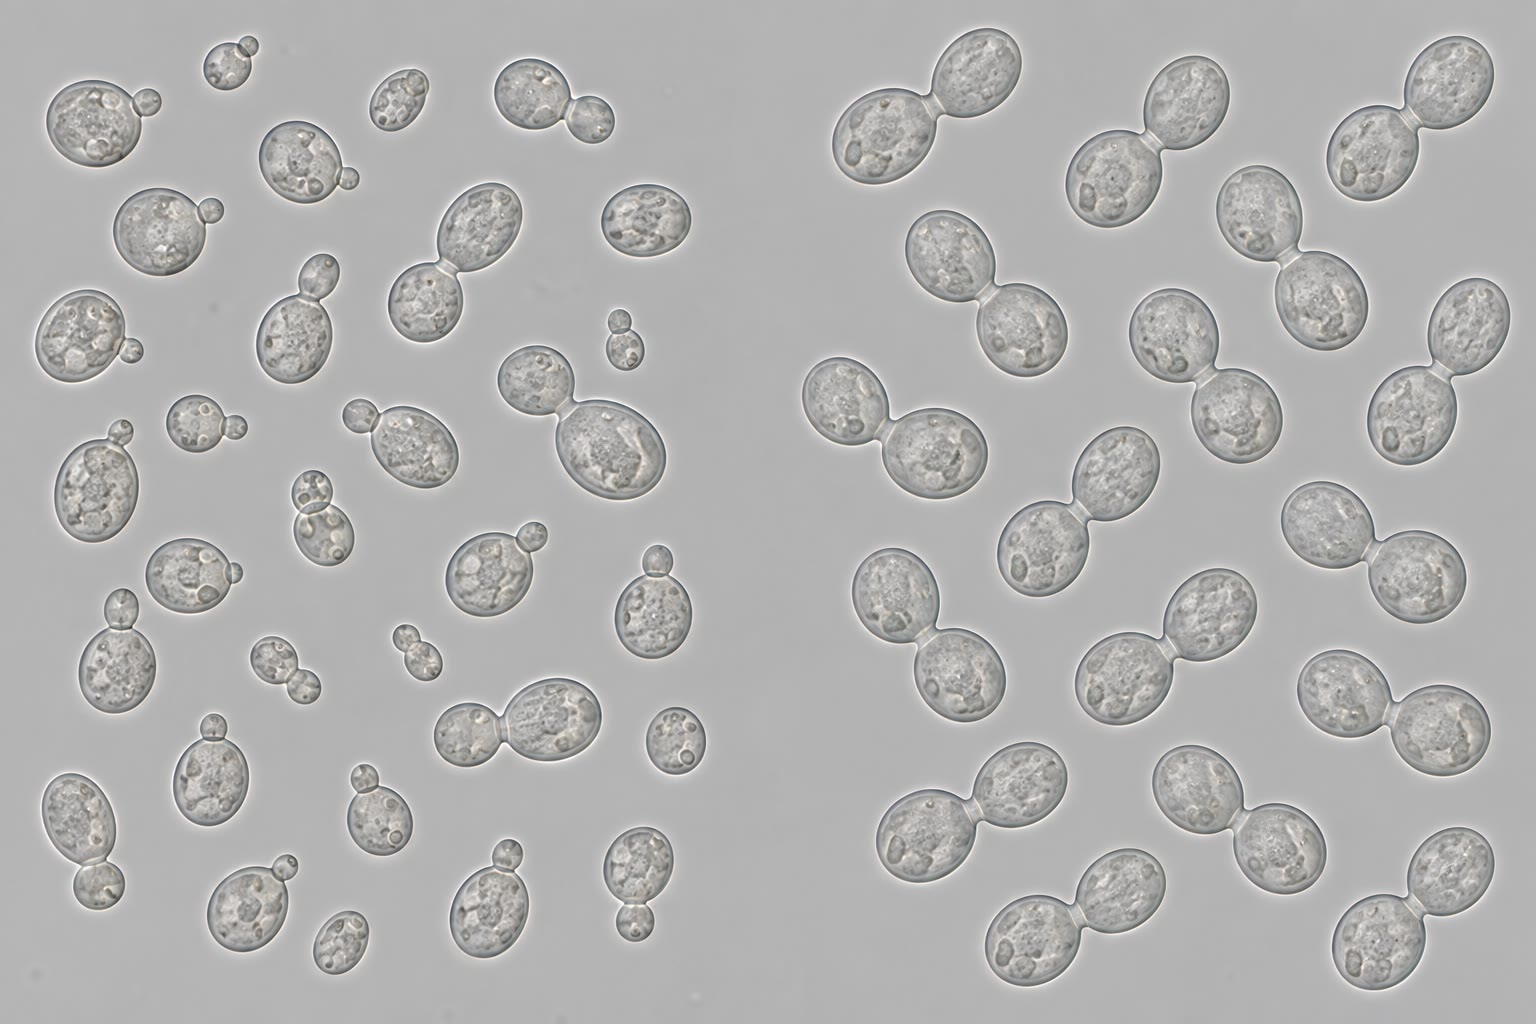
\includegraphics[width=0.54\linewidth]{images/book5/ai/b5-10-yeast-cdc-mutants.jpg}

{\small Links: een cel in de metafase --- \omterm{def:b3:cytoskeleton-motility:filaments}{microtubuli} van de
spoelfiguur (groen) vanaf de twee polen (rood), chromosomen (blauw)
uitgelijnd op de plaat, het ogenblik waarop het \omterm{def:b3:cell-cycle-apoptosis:checkpoints}{controlepunt van de
spoelfiguur} beslist. Rechts: bakkersgist, wildtype met knoppen van elke
grootte (links) en een \emph{cdc}-mutant waarin elke cel in hetzelfde
stadium is blijven staan, elk met een knop van dezelfde grootte
(rechts).}
\end{omfigure}

\section{Apoptose}

\begin{definition}[Apoptose]\label{def:b3:cell-cycle-apoptosis:apoptosis}
\index{apoptose}\index{necrose}\index{caspase}\index{fosfatidylserine}
\emph{Apoptose} is geprogrammeerde celdood volgens een inwendige reeks:
de cel krimpt en wordt rond, haar \omterm{def:b3:chromatin-epigenetics:nucleosome}{chromatine} verdicht zich en haar DNA
wordt tussen de \omterm{def:b3:chromatin-epigenetics:nucleosome}{nucleosomen} in een ladder van fragmenten geknipt, de
kern valt uiteen, het membraan blaast zich op tot afgesloten blaasjes,
fosfatidylserine verschijnt aan de buitenkant van het membraan als
``eet mij''-signaal, en de brokstukken worden binnen een uur door buren
of macrofagen verzwolgen --- zonder lekkage en dus zonder ontsteking.
Zij wordt uitgevoerd door \emph{caspasen}, cysteïneproteasen die achter
aspartaat knippen en als inactieve zymogenen worden gemaakt: de
\emph{initiatorcaspasen} (8 en 9) worden geactiveerd doordat zij op een
platform bijeen worden gebracht, en zij knippen en activeren de
\emph{beulscaspasen} (3 en 7), die enkele honderden substraten
doorknippen --- de lamines, het cytoskelet, de remmer van het
DNA-knippende nuclease, het enzym dat fosfatidylserine binnen houdt. De
\emph{necrose} is daarentegen dood door verwonding: de cel zwelt op,
barst, stort haar inhoud uit en wekt ontsteking op. De apoptose werd
benoemd en haar vorm beschreven door Kerr, Wyllie en Currie (1972);
haar genen werden in een worm gevonden.
\end{definition}

\begin{proof}[Bewijsmateriaal]
Elke hermafrodiet van \emph{Caenorhabditis elegans} maakt $1090$
somatische cellen, waarvan dezelfde $131$ sterven, elk op een vast
tijdstip en een vaste plaats. Horvitz en collega's (jaren tachtig)
isoleerden mutanten waarin zij overleefden: \emph{ced-3} en
\emph{ced-4} waren voor elke dood nodig, en zonder hen leefden en
differentieerden de $131$ cellen; \emph{ced-9} beschermde --- het
verlies ervan doodde cellen die hadden moeten leven, een te grote
werkzaamheid ervan redde cellen die hadden moeten sterven;
\emph{egl-1} was voor bepaalde sterfgevallen nodig. CED-3 was een
\omterm{def:b3:cell-cycle-apoptosis:apoptosis}{caspase}, CED-4 zijn activerende platform (Apaf-1 bij de mens), CED-9
een Bcl-2-eiwit, EGL-1 een BH3-only-eiwit: de menselijke route, gen
voor gen. Het menselijke gen \emph{BCL2} was zelf gevonden bij een
chromosoomtranslocatie in het folliculair lymfoom, een kanker van
cellen die niet sterven.
\end{proof}

\begin{definition}[De twee routes]\label{def:b3:cell-cycle-apoptosis:pathways}
\index{intrinsieke route}\index{extrinsieke route}\index{Bcl-2-familie}\index{cytochroom c}\index{apoptosoom}\index{doodsreceptor}
De \emph{intrinsieke} (mitochondriale) route brengt de inwendige
toestand van de cel samen. De \emph{Bcl-2-familie} kent drie klassen:
bewakers (Bcl-2, Bcl-xL, Mcl-1) die op het buitenmembraan van het
mitochondrion zitten en het gesloten houden; uitvoerders (Bax, Bak)
die zich, eenmaal geactiveerd, tot poriën in dat membraan
samenvoegen; en \emph{BH3-only}-sensoren (Bim, Bid, Puma, Noxa, Bad),
die elk door een bepaalde belediging worden aangezet of geactiveerd ---
DNA-schade via p53 (Puma, Noxa), het wegvallen van groeifactoren (Bim,
Bad), loslating, ongevouwen eiwitten --- en die de bewakers binden en de
uitvoerders vrijmaken of activeren. Winnen de uitvoerders, dan wordt
het buitenmembraan doorlaatbaar, lekt \emph{cytochroom~c} het cytosol
in, bindt het Apaf-1 en vormt het het \emph{apoptosoom}, dat \omterm{def:b3:cell-cycle-apoptosis:apoptosis}{caspase}~9
activeert. De \emph{extrinsieke} route begint buiten:
\emph{doodsreceptoren} (Fas, de TNF-receptor, de TRAIL-receptoren) die
door hun liganden op een doodlymfocyt of op een buurcel worden
gebonden, groeperen zich, trekken adaptoren aan en activeren \omterm{def:b3:cell-cycle-apoptosis:apoptosis}{caspase}~8,
dat \omterm{def:b3:cell-cycle-apoptosis:apoptosis}{caspase}~3 rechtstreeks knipt en, via Bid, ook de mitochondriale
weg opent. Beide routes komen samen op de beulscaspasen, en
remmereiwitten (IAP's, FLIP) stellen onderweg de drempel in.
\end{definition}

\begin{omfigure}
\begin{tikzpicture}[every node/.style={font=\scriptsize}, >=stealth]
  % extrinsic
  \node[draw, thick, rounded corners, fill=omProp!25, align=center] (lig) at (0,4.2) {doodsligand op een doodcel\\(FasL, TNF, TRAIL)};
  \node[draw, thick, rounded corners, fill=omProp!25, align=center] (rec) at (0,2.8) {doodsreceptoren groeperen zich;\\adaptoren trekken caspase-8 aan};
  \node[draw, thick, rounded corners, fill=omThm!20] (c8) at (0,1.5) {caspase-8 werkzaam};
  % intrinsic
  \node[draw, thick, rounded corners, fill=omDef!20, align=center] (insult) at (7.2,4.2) {DNA-schade (p53), verlies van groeifactor,\\loslating, ongevouwen eiwitten};
  \node[draw, thick, rounded corners, fill=omDef!20, align=center] (bh3) at (7.2,3.0) {BH3-only-sensoren (Puma, Bim, Bid)\\schakelen Bcl-2 uit, activeren Bax/Bak};
  \node[draw, thick, rounded corners, fill=omDef!20, align=center] (mito) at (7.2,1.7) {buitenmembraan van het mitochondrion opent:\\cytochroom $c$ eruit, apoptosoom vormt zich};
  \node[draw, thick, rounded corners, fill=omThm!20] (c9) at (7.2,0.5) {caspase-9 werkzaam};
  % convergence
  \node[draw, thick, rounded corners, fill=omThm!35, align=center] (c3) at (3.6,-0.8) {beulscaspasen 3 en 7:\\honderden substraten doorgeknipt};
  \node[draw, thick, rounded corners, fill=gray!15, align=center] (out) at (3.6,-2.3) {chromatine verdicht, DNA in een ladder, blaasvorming,\\fosfatidylserine blootgelegd, verzwolgen};
  \draw[->, thick] (lig) -- (rec); \draw[->, thick] (rec) -- (c8); \draw[->, thick] (c8) -- (c3);
  \draw[->, thick] (insult) -- (bh3); \draw[->, thick] (bh3) -- (mito); \draw[->, thick] (mito) -- (c9); \draw[->, thick] (c9) -- (c3);
  \draw[->, thick] (c3) -- (out);
  \draw[->, thick, dashed] (c8) -- (bh3) node[pos=0.55, below, sloped] {Bid geknipt: de twee wegen komen samen};
  \node[left, omThm, align=right] at (-2.3,1.5) {extrinsieke\\route}; \node[right, omDef, align=left] at (10.4,1.7) {intrinsieke\\route};
  \node[right, font=\tiny, align=left] at (8.6,0.5) {IAP's remmen hier;\\Bcl-2 bewaakt hierboven};
\end{tikzpicture}

{\small De twee wegen naar de beulscaspasen. Van buiten naar binnen
activeert een \omterm{def:b3:cell-cycle-apoptosis:pathways}{doodsreceptor} caspase-8; van binnen naar buiten weegt de
\omterm{def:b3:cell-cycle-apoptosis:pathways}{Bcl-2-familie} de toestand van de cel en, wanneer de uitvoerders winnen,
laat het mitochondrion cytochroom~$c$ los en wordt caspase-9
geactiveerd. Beide komen samen op caspase-3.}
\end{omfigure}

\begin{proposition}[Het punt van geen terugkeer]\label{prop:b3:cell-cycle-apoptosis:mompt}
\index{permeabilisatie van het mitochondriale buitenmembraan}
Het doorlaatbaar worden van het buitenmembraan van het mitochondrion
gebeurt plotseling --- alle mitochondriën van een cel gaan binnen
ongeveer vijf minuten open, na uren van beraad --- en volledig: zodra
cytochroom~$c$ in het cytosol is, volgt de activering van de \omterm{def:b3:cell-cycle-apoptosis:apoptosis}{caspasen}
binnen minuten en is zij niet ongedaan te maken door de prikkel weg te
nemen. Twee kenmerken maken er een schakelaar van. De Bax/Bak-porie
ontstaat door samenvoeging, zodat haar snelheid steil stijgt met de
hoeveelheid geactiveerde uitvoerder; en de bewakers en sensoren binden
elkaar met hoge affiniteit, zodat tot een drempel elke sensor wordt
uitgeschakeld en daarboven elke extra sensor vrij is --- een titratie,
als een buffer die uitgeput raakt. De cel sterft daarom niet
geleidelijk; zij stapelt BH3-only-eiwitten op tot een drempel wordt
overschreden, en sterft dan in één keer. Geneesmiddelen die
BH3-eiwitten nabootsen (venetoclax, dat Bcl-2 bezet) duwen cellen die
zijn ``voorgeladen'' --- al dicht bij de drempel, zoals veel
leukemiecellen --- eroverheen, en sparen cellen die dat niet zijn.
\end{proposition}

\begin{omfigure}
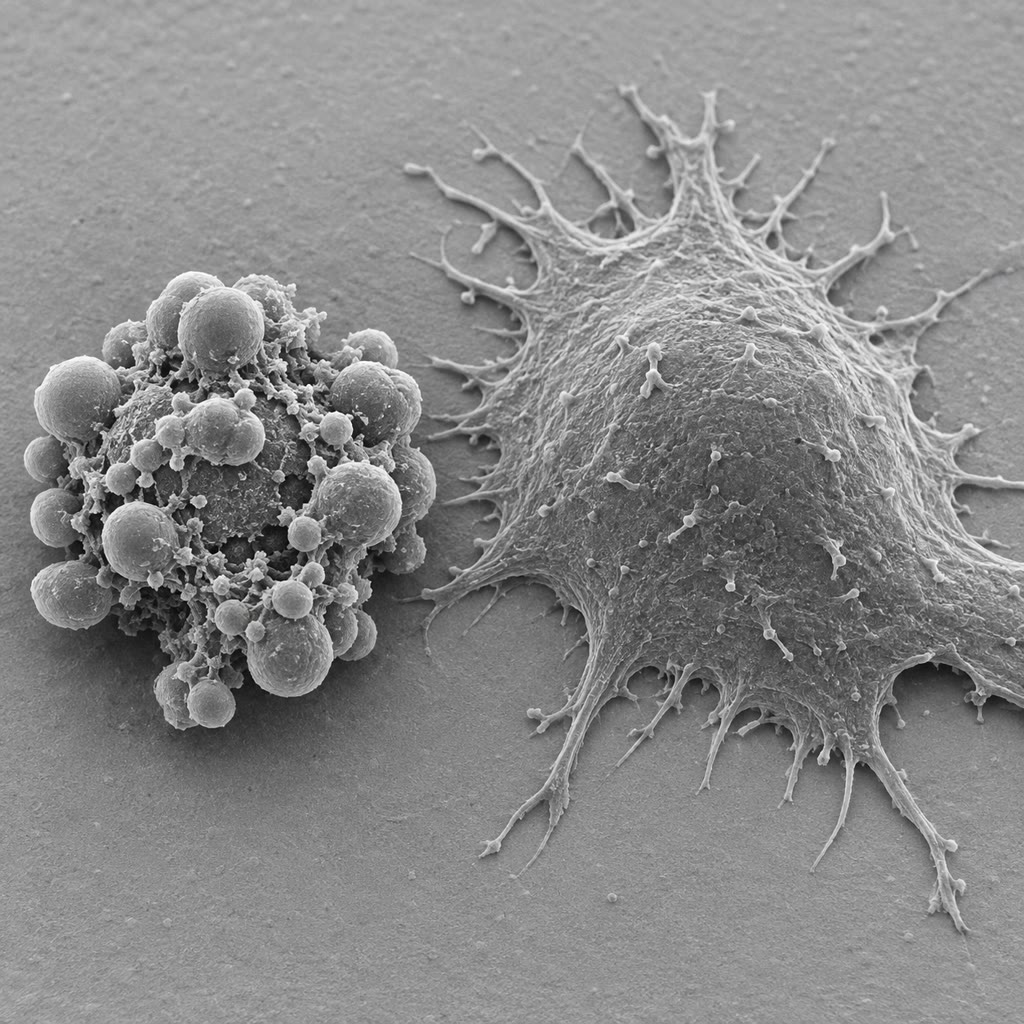
\includegraphics[width=0.40\linewidth]{images/book5/ai/b5-10-apoptotic-cell.jpg}

{\small Een apoptotische cel naast een gezonde in de
rasterelektronenmicroscoop: geslonken, met haar oppervlak opgebroken in
afgesloten blazen die zonder enig spoor van ontsteking zullen worden
verzwolgen.}
\end{omfigure}

\begin{example}[Sterfgevallen die een lichaam bouwen]\label{ex:b3:cell-cycle-apoptosis:development}
De vingers worden uit een peddel gesneden door de \omterm{def:b3:cell-cycle-apoptosis:apoptosis}{apoptose} van de
cellen ertussen; bij de eend leven diezelfde cellen en blijft het vlies
zitten. De staart van het kikkervisje wordt bij de gedaanteverwisseling
op het signaal van schildklierhormoon geresorbeerd. Ongeveer de helft
van de neuronen die in het zenuwstelsel van een gewervelde worden
gemaakt sterft vóór de geboorte, namelijk die welke onvoldoende
trofische factor van hun doelwitten ontvangen --- een wedijver die het
aantal neuronen afstemt op de omvang van het veld dat zij bedienen.
Vijfennegentig procent van de T-cellen die in de thymus worden gemaakt
sterft daar, weggeselecteerd omdat zij niets herkennen of het eigene
herkennen (\cref{ch:b3:adaptive-immunity}). En elke dag stoot het
darmepitheel zijn oudste cellen af op de toppen van de villi, de huid
haar keratinocyten, en het bloed zijn verouderde neutrofielen na een
leven van een dag: de \omterm{def:b3:cell-cycle-apoptosis:apoptosis}{apoptose} is de gewoonte, en de omvang van een
weefsel is het verschil tussen twee grote snelheden.
\end{example}

\section{Andere uitgangen, en het uitblijven van de uitgang}

\begin{definition}[Gereguleerde necrose en senescentie]\label{def:b3:cell-cycle-apoptosis:other}
\index{necroptose}\index{pyroptose}\index{senescentie}
Cellen kennen nog andere geprogrammeerde sterfgevallen, alle
ontstekingsbevorderend waar de \omterm{def:b3:cell-cycle-apoptosis:apoptosis}{apoptose} zwijgt. De \emph{necroptose},
uitgelokt door \omterm{def:b3:cell-cycle-apoptosis:pathways}{doodsreceptoren} wanneer caspase-8 wordt geblokkeerd
(zoals sommige virussen doen), stelt het kinase RIPK3 samen met MLKL,
dat het plasmamembraan doorboort. De \emph{pyroptose}, in besmette
macrofagen, wordt uitgevoerd door caspase-1 van het inflammasoom
(\cref{ch:b3:innate-immunity}), dat gasdermine tot een porievormer
knipt en interleukine-1 vrijmaakt. De \emph{ferroptose} is dood door
ijzerafhankelijke lipideperoxidatie. Een cel kan ook ophouden met delen
zonder te sterven: de \emph{senescentie} is een blijvende stilstand,
afgedwongen door p16 en p21 na erosie van de telomeren
(\cref{ch:b3:stem-cells}), aanhoudende DNA-schade of activering van een
oncogen, waarbij de cel stofwisselend actief blijft en
ontstekingsfactoren uitscheidt. De senescentie haalt beschadigde
cellen uit de delende voorraad --- een tumoronderdrukker --- en neemt
met de leeftijd toe, waarbij haar uitscheiding bijdraagt aan de
aftakeling van weefsels; senescente cellen bij muizen opruimen verlengt
het gezonde leven.
\end{definition}

\begin{remark}[Te weinig en te veel]\label{rem:b3:cell-cycle-apoptosis:disease}
De ziekten van deze programma's zijn een kwestie van dosis. Te weinig
dood: kanker, waarbij de drempel voor \omterm{def:b3:cell-cycle-apoptosis:apoptosis}{apoptose} door overexpressie van
Bcl-2 of door verlies van p53 wordt verhoogd, zodat cellen met
beschadigde genomen overleven om nog meer schade op te stapelen;
auto-immuniteit, wanneer lymfocyten die in de selectie hadden moeten
sterven blijven bestaan. Te veel: het verlies van T-cellen bij een
hiv-infectie, de neuronen in de schemerzone van een beroerte die uren
na de ischemie door \omterm{def:b3:cell-cycle-apoptosis:apoptosis}{apoptose} sterven (een venster voor behandeling), de
trage \omterm{def:b3:cell-cycle-apoptosis:apoptosis}{apoptose} van neuronen bij neurodegeneratieve ziekten, de
hartcellen die na een hartinfarct verloren gaan. De behandeling van
kanker is grotendeels het opzettelijk opwekken van \omterm{def:b3:cell-cycle-apoptosis:apoptosis}{apoptose} in cellen
waarvan de drempels lager liggen dan die van hun buren, en de
geneesmiddelen die zich op Bcl-2 en Cdk4/6 richten zijn de eerste die
op de kaarten van dit hoofdstuk zijn ontworpen.
\end{remark}

\section{Opgaven}

\begin{exercise}[$\star$]\label{exo:b3:cell-cycle-apoptosis:1}
Noem de vier fasen van de cyclus, het paar van \omterm{def:b3:cell-cycle-apoptosis:cdk}{cycline} en CDK dat elke
overgang aandrijft, en het ubiquitineligase dat de mitose beëindigt.
\end{exercise}

\begin{exercise}[$\star$]\label{exo:b3:cell-cycle-apoptosis:2}
Wat droegen Hartwell, Nurse en Hunt elk bij aan de ontdekking van de
motor, en in welk organisme?
\end{exercise}

\begin{exercise}[$\star$]\label{exo:b3:cell-cycle-apoptosis:3}
Noem de drie \omterm{def:b3:cell-cycle-apoptosis:checkpoints}{controlepunten}, de voorwaarde die elk toetst en het
moleculaire doelwit waarop elk ingrijpt.
\end{exercise}

\begin{exercise}[$\star$]\label{exo:b3:cell-cycle-apoptosis:4}
Onderscheid \omterm{def:b3:cell-cycle-apoptosis:apoptosis}{apoptose} van \omterm{def:b3:cell-cycle-apoptosis:apoptosis}{necrose} in vijf kenmerken, en noem de
enzymklasse die de \omterm{def:b3:cell-cycle-apoptosis:apoptosis}{apoptose} uitvoert.
\end{exercise}

\begin{exercise}[$\star\star$]\label{exo:b3:cell-cycle-apoptosis:5}
In een extract van een kikkerei wordt \omterm{def:b3:cell-cycle-apoptosis:cdk}{cycline} B gemaakt met
$k_{s} = 1$ eenheid per minuut; de mitotische drempel is
$C_{2} = 30$ eenheden, de uitgangsdrempel $C_{1} = 5$, en in de mitose
wordt \omterm{def:b3:cell-cycle-apoptosis:cdk}{cycline} afgebroken met een halveringstijd van \qty{2}{min}. Schat
de periode van de oscillatie en het deel van de cyclus dat in de mitose
wordt doorgebracht.
\end{exercise}

\begin{exercise}[$\star\star$]\label{exo:b3:cell-cycle-apoptosis:6}
Voorspel het gedrag van een cel die (a) een niet-afbreekbaar \omterm{def:b3:cell-cycle-apoptosis:cdk}{cycline} B
tot expressie brengt, (b) Wee1 mist, (c) Cdc25 mist, (d) een Cdk1 tot
expressie brengt dat door Wee1 niet kan worden gefosforyleerd, in
termen van de oscillator uit
\cref{thm:b3:cell-cycle-apoptosis:oscillator}.
\end{exercise}

\begin{exercise}[$\star\star$]\label{exo:b3:cell-cycle-apoptosis:7}
Een fusie volgens Rao en Johnson voegt een cel in G1 en een cel in
S-fase samen; een andere voegt een cel in G2 en een cel in S-fase
samen. Voorspel wat elke kern doet en verklaar dat met de
\omterm{def:b3:cell-cycle-apoptosis:checkpoints}{replicatievergunning} en de CDK-niveaus.
\end{exercise}

\begin{exercise}[$\star\star$]\label{exo:b3:cell-cycle-apoptosis:8}
Leg uit waarom één enkele ongehechte kinetochoor de anafase voor de
hele cel kan tegenhouden, en voorspel het lot van een cel waarin Mad2
is verwijderd.
\end{exercise}

\begin{exercise}[$\star\star$]\label{exo:b3:cell-cycle-apoptosis:9}
Voorspel het fenotype van een worm zonder \emph{ced-9}; zonder
\emph{ced-3}; zonder beide. Verklaar de epistasie in termen van de
route.
\end{exercise}

\begin{exercise}[$\star\star\star$]\label{exo:b3:cell-cycle-apoptosis:10}
Laat zien dat één enkele negatieve terugkoppeling zonder bistabiele
schakelaar --- \omterm{def:b3:cell-cycle-apoptosis:cdk}{cycline} gemaakt met $k_{s}$, afgebroken met $k_{d}AC$
waarbij $A$ eenvoudig evenredig is met $C$ --- een stabiele
evenwichtstoestand heeft en niet oscilleert. Wat voegt de S-vormige
curve toe, en wat zou een vertraging in plaats daarvan toevoegen?
\end{exercise}

\begin{exercise}[$\star\star\star$]\label{exo:b3:cell-cycle-apoptosis:11}
Een cel heeft $N$ moleculen van de bewaker Bcl-2 en ontvangt na een
schadelijke prikkel BH3-only-sensoren met een snelheid $r$ per uur,
waarbij elke sensor één bewaker bindt. Leg uit waarom de cel omstreeks
tijdstip $N/r$ sterft, hoe sterk de prikkel daarboven ook is, waarom de
dood plotseling is, en wat venetoclax met die tijd doet.
\end{exercise}

\begin{exercise}[$\star\star\star$]\label{exo:b3:cell-cycle-apoptosis:12}
Het folliculair lymfoom draagt een translocatie die \emph{BCL2} tot
overexpressie brengt; de cellen delen zich traag. Het retinoblastoom
draagt het verlies van \emph{RB}; de cellen delen zich snel. Leg uit
hoe elk van beide enkelvoudige beschadigingen een tumor voortbrengt,
waarom de eerste sluimerend is en de tweede agressief, en wat elk zegt
over de twee programma's van dit hoofdstuk.
\end{exercise}

\section{Vraagstuk: leven en dood van een epitheel}

\begin{problem}[{Weekendvraagstuk --- de darmbekleding cel voor cel
vernieuwd, de cyclus getimed met de cyclineoscillator, de fouten van
een controlepunt over een heel lichaam geteld, en de apoptotische
opruiming van honderd miljard cellen per dag gewogen, met als besluit
de periode van de cyclus, het aantal aneuploïde cellen per dag en de
massa die het lichaam met apoptose hergebruikt}]
\label{pb:b3:cell-cycle-apoptosis:1}
Gegevens: de dunne darm heeft $10^{7}$ crypten, die elk om de $5$ dagen
een villus van \num{3500} cellen vernieuwen; elke crypte bevat ongeveer
$22$ stamcellen die zich eens per dag delen en waarvan het nageslacht
zich nog $5$ keer deelt voordat het differentieert. Oscillator:
$k_{s} = 2$ eenheden \omterm{def:b3:cell-cycle-apoptosis:cdk}{cycline} per uur, $C_{2} = 40$ eenheden,
$C_{1} = 8$, halveringstijd van mitotisch \omterm{def:b3:cell-cycle-apoptosis:cdk}{cycline} \qty{10}{min}.
\omterm{def:b3:cell-cycle-apoptosis:checkpoints}{Controlepunt}: zonder het \omterm{def:b3:cell-cycle-apoptosis:checkpoints}{controlepunt van de spoelfiguur} verdeelt één
deling op $50$ een chromosoom verkeerd; met dat \omterm{def:b3:cell-cycle-apoptosis:checkpoints}{controlepunt} één op
\num{50000}. Het lichaam vervangt $10^{11}$ cellen per dag met een
massa van \qty{1}{ng} elk, waarvan \qty{20}{\%} eiwit; een macrofaag
ruimt één apoptotische cel op in \qty{1}{h}.

\medskip
\noindent\textbf{Deel I --- Vernieuwing.}
\begin{enumerate}
  \item Hoeveel cellen stoot de dunne darm per dag af, en per seconde?
  \item Hoeveel cellen maakt één crypte per dag? Controle: $22$
        stamceldelingen per dag, waarbij elke vastgelegde dochter zich
        nog $5$ keer deelt.
  \item Als een stamcel zich een leven van $80$ jaar lang eens per dag
        deelt, hoeveel delingen zijn dat? Hoeveel mutaties stapelt zij
        op bij een mutatiesnelheid van $0.6$ per genoom per deling
        (\cref{ch:b3:dna-repair})?
  \item De transitcellen delen zich elke \qty{12}{h}. Waarom kan het
        weefsel zich snelle, kortlevende transitdelingen veroorloven
        maar houdt het de stamcel traag?
  \item Een stralingsdosis doodt alle delende transitcellen maar spaart
        de stamcellen, die zich binnen een dag herstellen. Hoe lang
        duurt het voordat de villus, zonder aanvulling, kaal is, en hoe
        lang duurt de heropbouw? Waarom is de darm een vroeg
        slachtoffer van straling?
  \item In de dikke darm gebeurt het afstoten aan de top door \omterm{def:b3:cell-cycle-apoptosis:apoptosis}{apoptose}
        (anoikis, dood bij loslating). Waarom is dat de juiste vorm van
        dood voor een cel die in aanraking is met darmbacteriën?
\end{enumerate}

\medskip
\noindent\textbf{Deel II --- De klok.}
\begin{enumerate}[resume]
  \item Hoe lang doet \omterm{def:b3:cell-cycle-apoptosis:cdk}{cycline} er volgens de gegevens van de oscillator
        over om van $C_{1}$ tot $C_{2}$ te stijgen?
  \item Hoe lang doet de mitotische afbraak erover om het van $C_{2}$
        terug op $C_{1}$ te brengen?
  \item Wat is de periode van de kale oscillator, en welk deel van de
        periode is Cdk1 werkzaam?
  \item De transitcellen van de crypte doorlopen hun cyclus in
        \qty{12}{h}, de stamcellen in \qty{24}{h}, het kikkerei in
        \qty{30}{min}. Welke parameter van het model verschilt, en wat
        levert het verschil in een somatische cel?
  \item Een cel die door DNA-schade bij het \omterm{def:b3:cell-cycle-apoptosis:checkpoints}{controlepunt} G2/M is
        stilgezet blijft \omterm{def:b3:cell-cycle-apoptosis:cdk}{cycline} B maken. Waar zit zij op het faseplat,
        en wat houdt haar daar? Wat gebeurt er wanneer de schade is
        hersteld?
  \item Een geneesmiddel remt het APC/C. Beschrijf het lot van een cel
        die in zijn aanwezigheid de mitose ingaat.
\end{enumerate}

\medskip
\noindent\textbf{Deel III --- Fouten.}
\begin{enumerate}[resume]
  \item Hoeveel delingen per dag voert het lichaam uit om $10^{11}$
        cellen te vervangen?
  \item Hoeveel aneuploïde dochters per dag met het \omterm{def:b3:cell-cycle-apoptosis:checkpoints}{controlepunt}, en
        hoeveel zonder?
  \item De meeste aneuploïde cellen sterven of komen stil te staan (p53
        reageert op een verkeerde verdeling). Hoeveel aneuploïde
        delende cellen maakt een lichaam met een werkend \omterm{def:b3:cell-cycle-apoptosis:checkpoints}{controlepunt}
        per dag, en over een heel leven, als \qty{1}{\%} overleeft en
        zich deelt?
  \item Een tumor van $10^{9}$ cellen heeft het \omterm{def:b3:cell-cycle-apoptosis:checkpoints}{controlepunt} en p53
        verloren. Hoeveel verkeerde verdelingen voert zij per dag uit,
        en waarom evolueert zij daardoor snel?
  \item Leg uit waarom het volledige verlies van het \omterm{def:b3:cell-cycle-apoptosis:checkpoints}{controlepunt van de
        spoelfiguur} dodelijk is voor een embryo terwijl gedeeltelijk
        verlies kanker bevordert.
  \item Het downsyndroom ontstaat door een verkeerde verdeling in de
        meiose en niet in de mitose. Leg uit waarom een fout in één cel
        daar elke cel van het kind treft, terwijl één mitotische fout
        één afstammingslijn treft.
\end{enumerate}

\medskip
\noindent\textbf{Deel IV --- Opruiming.}
\begin{enumerate}[resume]
  \item Welke massa cellen ruimt het lichaam per dag met \omterm{def:b3:cell-cycle-apoptosis:apoptosis}{apoptose} op, en
        per jaar? Vergelijk met de lichaamsmassa.
  \item Hoeveel eiwit is dat per dag? Vergelijk met een voedselinname
        van \qty{70}{g}: welk deel van de eiwitomzet van het lichaam is
        het hergebruik van dode cellen?
  \item Hoeveel macrofagen zijn er, onafgebroken werkend, nodig om de
        dagelijkse doden op te ruimen? Het lichaam heeft ongeveer
        $10^{11}$ macrofagen: welk deel van hun tijd is dat?
  \item Waarom moet het lijk worden weggehaald voordat het uiteenvalt,
        en wat geeft het signaal ``eet mij''?
  \item Bij een patiënt komt Bcl-2 in de B-cellen tot overexpressie.
        Welke route is geblokkeerd, werkt de \omterm{def:b3:cell-cycle-apoptosis:pathways}{extrinsieke route} nog, en
        waarom is het resultaat een traag groeiend lymfoom en geen snel
        groeiend?
  \item Neuronen in de schemerzone van een beroerte sterven zes tot
        vierentwintig uur na de beschadiging door \omterm{def:b3:cell-cycle-apoptosis:apoptosis}{apoptose}, die in de
        kern binnen minuten door \omterm{def:b3:cell-cycle-apoptosis:apoptosis}{necrose}. Waarom biedt het eerste een
        venster voor behandeling en het tweede niet?
  \item Vat samen: de periode van de kale oscillator (vraag~9), het
        aantal aneuploïde delende cellen per dag in een normaal lichaam
        (vraag~15), en de massa die per dag met \omterm{def:b3:cell-cycle-apoptosis:apoptosis}{apoptose} wordt
        hergebruikt (vraag~19).
\end{enumerate}
\end{problem}
